% -*- TeX-master: t -*-
\documentclass[12pt,letterpaper]{article}

% acmart already includes: graphicx, hyperref, booktabs, amsmath, natbib
% Only load packages not included in acmart

\usepackage{csquotes}
\usepackage{subcaption}
\usepackage{siunitx}
\usepackage{tikz}
\usepackage{listings}
\usepackage{xcolor}
\usepackage[ruled,vlined]{algorithm2e}
\usepackage{cleveref}

% Configure cleveref for algorithm2e
\crefname{algocf}{Algorithm}{Algorithms}

\usetikzlibrary{positioning, shapes, arrows.meta, fit, backgrounds}
\lstset{
    basicstyle=\ttfamily\footnotesize,
    breaklines=true,
    frame=single,
    numbers=left,
    numberstyle=\tiny\color{gray},
    keywordstyle=\color{blue},
    commentstyle=\color{green!60!black},
    stringstyle=\color{red},
    showstringspaces=false,
    captionpos=b,
    inputencoding=utf8,
    extendedchars=true,
    literate={·}{{\textperiodcentered}}1 {−}{{\textminus}}1 {—}{{---}}1 {–}{{--}}1
}

% Use biblatex instead of natbib (acmart default)
\usepackage[backend=bibtex,style=numeric]{biblatex}
\addbibresource{bib/references.bib}


\begin{document}

\begin{titlepage}
    \centering
    
\includegraphics[width=\textwidth]{graphics/banner.png}\\[0.8cm]
    \LARGE\textbf{PHANTOM: Pricing Heuristics Against Non-human Transaction Orchestration Mechanisms}\\[0.5cm]
    \Large\textbf{Daniel Rösel}\\
    \large\textit{Bachelor of Computer Science \& Artificial Intelligence}\\[0.5cm]
    \Large\textit{Supervised by:}\\
    \Large\textbf{Alberto Martín Izquierdo}\\
    \large\textit{IE University, Madrid, Spain}\\[1cm]
    \large\today
\end{titlepage}

\begin{abstract}
\noindent
Large language model (LLM) agents are spreading in e-commerce; one consequence is intermediaries that can separate information gathering from transaction execution. This thesis studies dynamic pricing when agents reconnoitre in isolated sessions and thereby weaken the \emph{Cost of Information} (COI), the premium platforms typically extract once demand signals are expressed.

We formalize the phenomenon and prove a Cost of Information theorem: as independent, utility-maximizing agents saturate price queries, the platform's sustainable COI goes to zero, so ordinary dynamic pricing is incentive-incompatible in the limit.

The defensive design combines behavioral signals with distributionally robust optimization (DRO). We implement a controlled storefront on a hybrid Kappa--Lambda architecture and show that human and agent sessions induce different transition kernels. Kullback--Leibler divergence to class prototypes yields session scores that feed a distributionally robust reinforcement learning (DR-RL) policy, posed as a Stackelberg game with a Wasserstein ambiguity set over demand so the learner does not collapse to a single empirical demand curve under shifting contamination.

Factorial training on TPUs shows the expected short-run revenue hit from contamination and that the robust objective recovers COI and equilibrium structure in harder regimes (higher contamination, larger catalogs), accounting for UX to prevent supra-competitive pricing. Code and an interaction dataset are released for work on agent-mediated traffic.
\end{abstract}

\noindent\textbf{Keywords:} Dynamic Pricing, LLM Agents, Adversarial Machine Learning, E-commerce, Behavioral Detection, Reinforcement Learning

\vspace{0.5em}
\noindent\textbf{Project page:} \url{https://velocitatem.github.io/PHANTOM/}

\clearpage
%% Cite like this \parencite{knuth1984texbook}. See \cref{fig:example}.
%% \begin{figure}[h]
%%   \centering
%%   \includegraphics[width=.7\linewidth]{figures/example.pdf}
%%   \caption{Example figure.}
%%   \label{fig:example}
%% \end{figure}

\section{Introduction}

Research Objectives and Contribution: What are we making, why and who should care?

\subsection{Motivation and Market Context}
Current market dynamics and trends of dynamic pricing and AI agents. Future projections of AI agents. Key stakeholders that are discussing this and reporting on it (Thales). Who is most affected
\subsection{Solution Space Overview}
Different approaches and perspectives, here also add a preview of what will be developed and explored in the lit review.

\section{Literature Review}


\subsection{Agent Taxonomy and Definitions}

describe agents as defined in \cite{Russell}

\subsection{Economic Agents: From Homo Economicus to Machina Economicus}

Existing behvarioal economic models tend to be criticized for the assumption of rational behavior, as is embodied in the term of homo economicus. The definition of a machina economicus by \cite{Parkes2015} is quite apropriate for our case...
What is the taxonomy and definition of an agent and an actor in this case, a bit more about interaction models in sessions and about dynamic pricing algorithms.

\subsection{Problem Evidence and Market Impact}
Documented instances of agent-driven market disruptions - Quantitative evidence of pricing manipulation - Case studies from affected industries

\subsection{Theoretical Foundations: Economic Prallels}

Economic foundations: relating the problem to options pricing theory. Cost of Information (COI) concept and its relevance

\subsection{Landscape of Existing Work}

Previous efforts in adversarial computer use LLM agents, show how multi-faceted the whole problem is
Here we can show a market visualization (venn-like-diagram)

\section{Methodology}

\subsection{Problem Formalization}

Mathematical formalization of agent-induced pricing distortions. Formal definition of potential loss mechanisms $\alpha D$

We consider a business across time during which we have an evolving vector $p_t \in \Re^N$ where $N$ is the number of products in our catalogue. our price vector is directly dependent on a demand function $q_t$ which we define as a linear method of a price elasticity matrix $B_t$. This is the same setup that Microsoft created in their research.

We gether interaction data from users interacting with a sample platform simulating a hotel/airline which generates interaction distributions $I_t = \{(p_t, q_t^\text{obs}, \pi_t)\}_{t=1}^T$


\subsection{Cost of Information Framework}

Mathematical demonstration and validation of the COI and citation backed evidence, and framework overview + show harm to user via other cost distortions. Maybe split into 3.2.1 (COI Theory) and 3.2.2 (Framework Design)

\subsection{System Architecture}

In order for our research to have grounding in interactions we built a robust e-commerce web-platform. We initially conducted a survey of the leading platforms of airlines and hotel booking sites to identify the specific interface patterns that effectively manage complex travel data. Our analysis revealed a clear industry standard: while both sectors rely on tabbed service selection and left-sidebar filtering to streamline navigation, they diverge in result presentation—airlines utilize visual date-price bars and multi-step wizards to optimize for logistical transparency, whereas hotel platforms leverage image-led cards and scarcity triggers to drive emotional engagement and urgency. Our web framework defines a highly agnostic boilerplane which can be seeded with any data-modality with an easy-to-tailor pattern, which we leverage to define a \texttt{hotel} and \texttt{airline} mode. Both modes are then individually deployed via an envrionment level argument which adjusts the proxy routing with a custom middleware inside next.js to render only the desired mode. The purpose of this was to create a baseline adaptable to any use-case or desired commercial application.




\subsection{Experimental Design}

\begin{figure}[ht]
  \resizebox{\columnwidth}{!}{%
    \definecolor{mygreenfill}{RGB}{169, 234, 186}
\definecolor{mygreenborder}{RGB}{29, 145, 61}
\definecolor{mybluefill}{RGB}{204, 222, 255}
\definecolor{myblueborder}{RGB}{66, 106, 189}
\definecolor{mygray}{RGB}{150, 150, 150}



\begin{tikzpicture}[
    node distance=2cm,
    % Style for Green Nodes
    greenbox/.style={
        rectangle,
        draw=mygreenborder,
        fill=mygreenfill,
        line width=1.2pt,
        align=center,
        minimum height=1cm
    },
    % Style for Blue Nodes
    bluebox/.style={
        rectangle,
        draw=myblueborder,
        fill=mybluefill,
        line width=1.2pt,
        align=center,
        minimum height=1cm
    },
    % Style for Arrows
    myarrow/.style={
        ->,
        >={Stealth[length=3mm, width=2mm]},
        draw=black!80,
        line width=1.2pt,
        rounded corners=5pt
    },
    % Style for Background Dashed Circles
    dashedloop/.style={
        dashed,
        draw=mygray,
        line width=1pt
    }
]

    % --- Coordinate Layout ---
    % Defining a grid relative to the center

    % Left Loop (Green) Nodes
    \node[greenbox, minimum width=3.5cm] (commerce) at (-3.5, 2) {Commerce Experiment};
    \node[greenbox, minimum width=1.5cm] (raw) at (-6.5, 0) {Raw\\Logs};
    \node[greenbox, minimum width=1.5cm] (features) at (-4, -2.5) {Features};
    \node[greenbox, minimum width=2.5cm] (classification) at (-1, -0.5) {Classification\\Training A/H};

    % Right Loop (Blue) Nodes
    \node[bluebox, minimum width=2.5cm] (trainedpricing) at (3.2, 2) {Trained Pricing};
    \node[bluebox, minimum width=2.5cm] (policy) at (6.5, 0) {Trained Pricing\\Policy};
    \node[bluebox, minimum width=2.5cm] (rlgym) at (3.2, -2.2) {RL Gym\\Training};

    % --- Background Dashed Loops ---
    \begin{scope}[on background layer]
        % Left Loop Circle
        \draw[dashedloop] (-3.5, 0) ellipse (3.5cm and 2.8cm);
        % Right Loop Circle
        \draw[dashedloop] (3.5, 0) ellipse (3.5cm and 2.8cm);
    \end{scope}

    % --- Arrows: Loop One (Green) ---
    % Commerce -> Raw Logs
    \draw[myarrow] (commerce.west) to[out=180, in=90] (raw.north);

    % Raw Logs -> Features
    \draw[myarrow] (raw.south) to[out=270, in=180] (features.west);

    % Features -> Classification
    \draw[myarrow] (features.east) to[out=0, in=250] (classification.south);

    % Classification -> Commerce (Closing the loop)
    \draw[myarrow] (classification.north) to[out=110, in=0] (commerce.east);

    % --- Arrows: Loop Two (Blue) ---
    % Classification (Green) -> RL Gym (Blue) - Crossing over
    \draw[myarrow] (classification.east) to[out=0, in=180] (rlgym.west);

    % RL Gym -> Policy
    \draw[myarrow] (rlgym.east) to[out=0, in=270] (policy.south);

    % Policy -> Trained Pricing
    \draw[myarrow] (policy.north) to[out=90, in=0] (trainedpricing.east);

    % Trained Pricing -> Commerce (Crossing back)
    \draw[myarrow] (trainedpricing.west) -- node[above, font=\small, yshift=2pt] {New Pricing} (commerce.east);

    % --- Text Labels ---

    % Loop One Label
    \node[align=center] at (-3.8, 0) {Loop One:\\Data \textit{(Online)}};

    % Loop Two Label
    \node[align=center] at (3.5, 0) {Loop Two:\\Defense Gym \textit{(Offline)}};

    % Bottom Legend
    \node[font=\small] (taskA) at (-4, -4) {Dynamic Pricing Task A};
    \node[font=\small] (taskB) at (4, -4) {Dynamic Pricing Task B};
    \node[font=\small] (indep) at (0, -4) {Independent};

    % Arrows for bottom legend
    \draw[->, >=Stealth, thick, darkgray] (indep.west) -- (taskA.east);
    \draw[->, >=Stealth, thick, darkgray] (indep.east) -- (taskB.west);

\end{tikzpicture}

  }
  \caption{Overview of the Dynamic Pricing Tasks.}
\end{figure}
Study methodology and approach. Data acquisition strategy. Defined objectives and success criteria. Observable metrics and KPIs

\subsection{Dynamic Pricing Algorithm Analysis}
Deep dive into how the algorithm works, different kinds and justification for chosen appraoches + agent impact modeling and quantification.
\subsection{Reinforcement Learning Formulation}
How do we define the state space, action space and reward function breakdown and algorithm benchmarking.
POSSIBLY: Expand into full subsections: 3.6.1 (State-Action Space), 3.6.2 (Reward Design), 3.6.3 (Benchmarking)


\begin{algorithm}[t]
\DontPrintSemicolon
\KwIn{stepsize $\eta$, smoothing $\delta$, rank $d$}
\For{$t=1$ \KwTo $T$}{
  Sample $u_t$ on unit sphere; set $x_t^\prime=x_t+\delta u_t$\;
  Set $p_t \gets U x_t^\prime$ and observe $q_t, R_t(p_t)$\;
  $x_{t+1} \gets \Pi\_{\mathcal{X}}(x_t-\eta R_t(p_t) u_t)$\;
}
\caption{Online Pricing Optimization (template)}
\end{algorithm}

\section{Results}

\subsection{Behavioral Analysis}

Include markov chains of transition matrices, compare distributions (look at Divergence metrics)


\subsection{Experimental Outcomes}

Align with defined objectives, show results and statistical significance (or not).


\subsection{Interpretation and Insights}
Inference from given patterns and show key findings.

\subsection{Anomalies}

\section{Discussion}



\subsection{Transition to Agentic Market Microstructure}

Our analysis of the interaction dynamics between the platform and non-human actors suggests that the current static pricing models are insufficient for an agent-mediated economy. If we assume a transition toward a direct revelation mechanism, where actors must reveal their true valuation of a good through bidding dynamics, we inevitably introduce significant stochasticity into the pricing system. Unlike traditional e-commerce where prices are relatively sticky, such a mechanism implies a high volatility characteristic of financial equity markets (without the fungability however).

However, ecommerce commodities differ fundamentally from financial securities: they possess a hard floor defined by unit economics and reservation prices. The market might react enthusiastically to an iPhone priced at \$1, such a transaction is not permissible. The platform must establish an initial valuation anchor ($P_{0}$) defined by the marginal cost plus a target margin, around which the market price is permitted to fluctuate. We float the introduction of GenAI Agents as Institutional Market Makers. As the arms race for greater autonomy of agnetic systems grows, the commercial viability of AI agents has the potential to disseminate into every-day users directly interacting with them rather than e-commerce platforms. This is also under the assumption of expected transactional capabilities being given to AI Agents.



\subsection{Risk Assessment and Limitations}
\label{sec:limitations_risks}

This technology does not come without a more bitter side, ethical concerns do arise from the idea of deploying black-box like solutions to set prices based on a behavioral attributes. Approaches like universal behavioral profile modeling (UBPM) used in recommendation systems is very broadly utilized.

In our experimental setup we randomly assign each user to a platform and, within that platform, assign them to a task. Figure~\ref{fig:exp_design_tree} summarizes this design decision tree.

\begin{figure}[ht]
  \centering
  \resizebox{0.92\columnwidth}{!}{%
    % Horizontal tree: level distance must exceed ~half parent + half child width or nodes overlap (resizebox does not fix that).
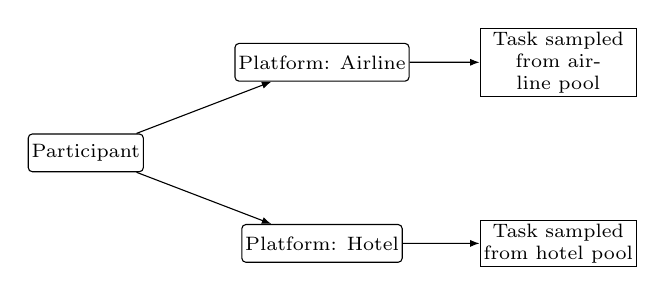
\begin{tikzpicture}[
  grow=right,
  level distance=30mm,
  sibling distance=23mm,
  decision/.style={
    rectangle,
    draw,
    rounded corners=1.5pt,
    align=center,
    inner sep=1.2pt,
    minimum width=14mm,
    minimum height=4.8mm,
    font=\scriptsize,
  },
  leaf/.style={
    rectangle,
    draw,
    align=center,
    inner sep=1.2pt,
    text width=19mm,
    minimum height=4mm,
    font=\scriptsize,
  },
  edge from parent/.style={draw, -{Latex[length=1.2mm]}},
]
\node[decision] {Participant}
  child {
    node[decision] {Platform: Hotel}
      child {node[leaf] {Task sampled\\from hotel pool}}
  }
  child {
    node[decision] {Platform: Airline}
      child {node[leaf] {Task sampled\\from airline pool}}
  };
\end{tikzpicture}

  }
  \caption{Experimental design decision tree for participant assignment.}
  \label{fig:exp_design_tree}
\end{figure}

Although our participant sample size is somewhat low for humans, we do a one-to-one balance of human-to-agent experimental sessions. This way we are observing a uniform distribution of participation from each participating side. Our sample size of participants might look scarce, but each participant generates a rich amount of data, with a totality of 3,874 rows of data.

With a system like this there is potential for strong drift given the rapid advance of agentic systems and user preference. Our intent behind adding the UX term into the reward shaping process was to further address the risk of degraded user experience. Looking deeper at the underlying methodology, reinforcement learning does not come without it's complications such as reward hacking and often the lack of intepretability which is quite critical in systems that have a strong impact on the revenue of a company.

% \subsection{Implications of Findings} Interpretation of results and altenrative scenarios with broader market implications.

\section{Conclusion}
\label{sec:conclusion}

This thesis examined reinforcement-learning policies for dynamic pricing when a fraction of traffic is orchestrated by non-human agents intent on extracting information before purchase. We introduced COI-oriented metrics, a behavioral distinguishability layer, and a distributionally robust training loop, empirical runs show where robustness helps and where it must be tuned.

\subsection{Summary of contributions}
Our work has yielded a broad set of dependencies which we carefully orchestrated to give us measurable results. To give a clear picture we outline the specific contributions of each stage of our work. The theoretical component formalizes why agent-mediated reconnaissance erodes pricing power, the behavioral component establishes that such contamination is detectable from interaction traces alone, the control component translates that distinguishability into a robust pricing mechanism, and the systems component provides the controlled experimental environment required to observe, test, and reproduce these effects.

\begin{itemize}
    \item TPU-accelerated parallelization of the behavioral simulation and reinforcement learning pipeline, making large factorial sweeps tractable.
    \item Formalization of non-human transaction orchestration in e-commerce as a distinct source of contamination in dynamic pricing systems.
    \item Definition of the Cost of Information (COI) as a mechanism-level quantity for pricing power, together with a theorem on its erosion under increasing agent saturation.
    \item Design and implementation of a controlled e-commerce research platform on a hybrid Kappa--Lambda architecture for collecting and replaying high-fidelity interaction trajectories.
    \item Construction and empirical validation of a behavioral distinguishability framework that separates human and agent sessions from interaction signals alone using transition kernels and KL-based divergence.
    \item A generative contamination mechanism that injects learned agent behavior into the pricing environment for controlled robustness experiments.
    \item Translation of distinguishability scores into defensive pricing via distributionally robust reinforcement learning under non-stationary contamination.
    \item Evidence that contamination depresses revenue and that robustness gains are regime-dependent, so penalties and radii need calibration rather than a single default.
    \item Release of a public experimental artifact (code and dataset) for reproducing and extending work on agent-mediated traffic.
\end{itemize}

\subsection{Limitations and future work}

Several constraints are intentional and could be relaxed later. Action weights in the demand proxy are currently derived from simple divergence rankings, learning them from data is an obvious next step. We propose a jointly learn the demand proxy, policy, and simulator parameters instead of treating them modularly. Another avenue we could not cover in this work is incorporating Bayesian methods better capture demand uncertainty and propagation of that uncertainty into reward systems.
The Stackelberg interface assumes a clean alternation between platform move and market response. Richer histories (multi-agent, multi-platform) would need a less rigid state definition. Non-perishable catalog supply in the simulator widens the sim-to-real gap for inventory-constrained domains. Within-session contamination is modeled as stable, time-varying $\alpha$ inside a session would better match some attack patterns.

Before any deployment, human baselines should grow beyond the convenience sample used here, catalog scaling laws should be re-checked when transition matrices grow with SKU count, and the full pipeline should be re-validated under production traffic volumes, governance constraints, and product mixes.
We conclude our work with enthusiasm for future developments in the field of agent mediated commerce, we are excited to provide the foundations for these developments and hope to see future work in similar spirit.


\section*{Acknowledgements}

This research was supported by the TPU Research Cloud program, which provided access to Google Cloud Tensor Processing Unit (TPU) accelerators, including TPU v4, v5e, and v6e.

I am grateful to Marco Casalaina (VP of Product, Core AI, Microsoft) for an early conversation on dynamic pricing that helped frame the problem. Eugene Bykovets (Ph.D.) pointed out useful parallels with blockchain systems and the difficulty of inferring intent under pseudonymity. Alberto Mart\'{i}n Izquierdo supervised this work and accepted an unusually wide brief. Several peers contributed through discussion of the topics covered here. The head of innovation at Amadeus offered industry perspective on margin compression under automation.

Generative tools were used for literature search, prototyping, and drafting support; all claims, experiments, and final wording remain the author's responsibility.


\printbibliography

\clearpage
\appendix
\section{Terminology}
\begin{description}
\item[Agent $A$] A non-human actor, typically an LLM-driven system that executes web actions toward a goal.
\item[Human $H$] A human participant interacting with the platform to complete a task.
\item[Actor Class $Y$] A latent class parameter describing whether a session is generated by a human or an agent profile.
\item[Platform] A web interface exposing purchasable items and their offered prices.
\item[Session $s$] A bounded interaction record tied to one actor and one session identifier.
\item[Event $e_{s,k}$] A single interaction tuple in a session, including action, item target, and timestamp.
\item[Trajectory $\tau_s$] The ordered sequence of events generated within a session.
\item[Demand Proxy $\hat{q}_{t,i}$] A weighted aggregate of observed actions used as an operational substitute for latent demand.
\item[Action Weight Function $\omega(a)$] A mapping from action type to signal strength in the demand proxy.
\item[True Demand $d(p\mid Y,\theta)$] The latent purchase response as a function of price, actor class, and latent type.
\item[Contamination $\alpha$] The proportion of agent-generated traffic in the session mixture.
\item[Non-stationary Noise $\epsilon_t$] Time-varying residual variation not explained by the actor mixture.
\item[Pricing Policy $\pi(\tau)$] A function mapping observed interaction history to an offered price.
\item[Cost of Information (COI)] The expected premium above the minimum viable price induced by the pricing policy.
\item[COI Leakage] A per-quote penalty term modeling information revealed to reconnaissance behavior.
\item[First-Order Statistic $p_{(1)}$] The minimum observed price among multiple independent queries.
\item[Transition Kernel $\mathcal{T}$] A Markov transition matrix over behavioral states or actions.
\item[Distinguishability] The degree to which human and agent sessions can be distinguished from behavior alone.
\item[KL Divergence $D_{KL}$] A relative-entropy measure used to compare session transition structure against class prototypes.
\item[Divergence Scores $\Delta_H,\Delta_A$] Session-level distances to human and agent transition centroids.
\item[Weak Agent Probability $f(\tau)$] A session-level score estimating the likelihood that a trajectory is agent-generated.
\item[Contamination Generator $\mathcal{G}(\alpha)$] A simulator component that injects synthetic agent trajectories to reach a target mixture level.
\item[Stackelberg Game] A leader-follower formulation where the platform sets prices and demand responds.
\item[Ambiguity Set $\mathcal{U}_{\epsilon}$] A set of plausible demand distributions considered under distributional uncertainty.
\item[Wasserstein Ball] A distance-bounded neighborhood around an empirical distribution used in robust optimization.
\item[DR-RL] Distributionally Robust Reinforcement Learning for policies trained against worst-case distributional shifts.
\item[Nominal Contamination $\alpha_0$] The baseline contamination level around which robust candidates are evaluated.
\item[Robustness Radius $\epsilon_\alpha$] The local interval width used for inner minimization over contamination scenarios.
\item[Query-Tax Surrogate] A constant leakage proxy assigning fixed penalty to suspected reconnaissance queries.
\item[Revelation Surrogate] A leakage proxy based on $-\log\pi(p\mid\tau)$ to penalize highly informative quotes.
\item[Limbo Stack] The alternating game-history buffer that stores leader price moves and follower demand responses.
\item[UX Index] A bounded user-experience metric tracked to evaluate policy side effects on legitimate users.
\item[Look-to-Book Ratio] The ratio of search-like interactions to completed purchases, used as an operational contamination indicator.
\item[Hybrid Kappa-Lambda Architecture] A data design combining streaming ingestion with offline and batch learning loops.
\item[MDP / POMDP] Sequential decision models with full observability (MDP) or partial observability (POMDP).
\item[Behavioral Model] A model predicting what action is likely to follow from prior actions.
\item[LLM] Large Language Model served through an inference provider with tool-use capability.
\item[TPU] Tensor Processing Unit, a specialized accelerator architecture developed by Google.
\end{description}

\section{Aggregate Compute Budget Derivation}
\label{app:compute_budget}

The claimed peak throughput of approximately 160\,PFLOPS follows from multiplying the per-chip BF16 peak (from official Google Cloud TPU documentation) by the number of chips in each allocation tier and summing across generations.

\begin{table}[ht]
\centering
\caption{Per-generation contribution to aggregate BF16 throughput.}
\label{tab:compute_derivation}
\begin{tabular}{@{}lrrr@{}}
\toprule
\textbf{TPU Gen.} & \textbf{Chips} & \textbf{Peak BF16/chip (TFLOPS)} & \textbf{Subtotal (TFLOPS)} \\
\midrule
v6e (Trillium) & 128 & 918 & $128 \times 918 = 117{,}504$ \\
v5e            & 128 & 197 & $128 \times 197 = 25{,}216$  \\
v4             &  64 & 275 & $64  \times 275 = 17{,}600$  \\
\midrule
\textbf{Total} & \textbf{320} & & $\mathbf{160{,}320}$ \\
\bottomrule
\end{tabular}
\end{table}

Converting to petaFLOPS: $160{,}320\;\text{TFLOPS} = 160.32\;\text{PFLOPS} \approx 160\;\text{PFLOPS}$. This is the theoretical peak under sustained BF16 arithmetic; realized throughput depends on memory bandwidth utilization and inter-chip communication overhead, but the figure serves as a useful upper bound for provisioning decisions.



\section{KL divergence when the reference has zeros}
\label{app:kl_zeros}

The textbook definition $D_{\mathrm{KL}}(P\parallel Q)=\sum_k P(k)\log(P(k)/Q(k))$ is not usable as-is when our empirical reference puts $Q(k)=0$ somewhere the session distribution still visits: if $P(k)>0$ and $Q(k)=0$, that term wants to blow up to infinity. With only 29 sessions the estimated transition rows are incredibly sparse.

In code we do the basic fix: add a tiny floor $\varepsilon$ to both the numerator and denominator inside the log so nothing is exactly zero, which turns the sum into a finite, smoothed surrogate rather than a literal KL to raw counts. We also skip source states that do not exist at all in the reference kernel, because there is nowhere honest to compare against. This keeps the pipeline running and the divergence scores on a comparable scale, at the cost that the number is regularized KL behavior, not a purist information-theoretic quantity, which is acceptable here because we only use the gap between human-anchored and agent-anchored scores as a weak separability signal.


\section{Why the logarithm appears in the revelation surrogate}
\label{app:revelation_log}

Recall that $\text{COI}_{\text{leak}}(p,\tau') = f(\tau')\cdot\text{InfoValue}(p,\tau')$. The query-tax surrogate fixes $\text{InfoValue}$ to a positive constant: every suspected reconnaissance quote is penalized equally, which tracks the erosion theorem where independent query volume drives COI to zero. The revelation surrogate instead sets
\begin{equation}
\text{InfoValue}(p,\tau') = -\log \pi(p\mid\tau'),
\end{equation}
where $\pi(\cdot\mid\tau')$ is the pricing policy's distribution over quoted prices in context $\tau'$ (after whatever discretization or binning the engine uses).

For an outcome that occurs with probability $q$, the quantity $-\log q$ is the usual \emph{surprisal}: likely draws have small surprisal, rare draws have large surprisal. That is the same ``surprise'' people import into recommender systems when they formalize novelty as low predicted probability under a model---here the model is our own policy. The log is not decorative: it is the standard information-theoretic coding of ``how unexpected was this draw under $\pi$?'' In the reconnaissance reading, a quote from a thin slice of the policy's support is more identifying than a modal quote, because it pins down what the rule is willing to do in places where little mass sits.

Put together, the revelation form is \emph{contamination-weighted surprisal}: $f(\tau')$ scales how agent-like we judge the session, and $-\log\pi(p\mid\tau')$ scales how informative that realized price is relative to $\pi(\cdot\mid\tau')$. In implementation you still floor $\pi(p\mid\tau')$ away from zero so tail bins do not explode the penalty---the same honesty as Appendix~\ref{app:kl_zeros}: we use a regularized surrogate, not a literal infinite penalty.


% \input{../build/concatenated_code}

\end{document}
